\documentclass[11pt]{jarticle}

\usepackage{kws}
%%%%%%%% added by Keito Murata %%%%%%%%%%%%%%%
\usepackage{setspace}
\usepackage{bm}
\usepackage[dvipdfmx]{color}
\usepackage[dvipdfmx]{graphicx}
%\usepackage{amsmath}
%\usepackage{amsfonts}
\usepackage{relsize}
\usepackage{url}
\usepackage{algorithm}
\usepackage{algorithmic}
\newcommand{\nr}{\mathbb{R}_{\geq 0}}
\newcommand{\nc}{\mathbb{C}}
\newcommand{\nN}{\mathbb{N}}
\newcommand{\nrindex}{\mathbb{R}_{\scalebox{0.5}{$[0,1]$}}}
\newcommand{\lsum}{\mathsmaller{\sum}}
\renewcommand{\figurename}{Fig.}
\renewcommand{\tablename}{Table}
%--- \Hline definition ---%
\makeatletter
 \def\Hline{%
 \noalign{\ifnum0=`}\fi\hrule \@height 1.4pt \futurelet
 \reserved@a\@xhline}
\makeatother
%--- \Hline definition ---%
\renewcommand{\footnotesize}{\scriptsize}
%%%%%%%% added by Keito Murata %%%%%%%%%%%%%%%

\begin{document}
%
% もし、本文が英文ならば、日本語のタイトルと著者は不要です。
% その場合、下記の\OnlyEnglishtrueを有効にしてください。
% 英語のタイトルと著者のみを表示します。
% ただし、\jtitle, \jauthor, \jaddressの行は削字しないでください。
%\OnlyEnglishtrue


\jtitle{レーダセンサ及びブラインド信号源分離に基づく心拍推定}

\etitle{Heart Rate Estimation Based on Radar Sensor and Blind Source Separation}

\jauthor{村田佳斗$^{\dag}$ \hspace{2cm} 北村大地$^{\ddag}$}

\eauthor{Ichiro TSUSHIN$^{\dag}$ \hspace{2cm} Taro KARUIZAWA$^{\ddag}$}

\jaddress{\dag 香川高等専門学校 \\ \ddag (株) 信濃電子システム研究所}

\eaddress{\dag Denshi University \\ \ddag Shinano Denshi Corp.}


\maketitle

\section{はじめに}
\hspace{1em}自動車の運転中に運転者が睡眠,突発的な発作,体調の悪化による意識喪失等に見舞われることは多くの場合致命的な状況となる.そのため,運転中に運転者の状態を何らかの方法で管理することが重要課題の一つとなっている.

この課題に取り組むために,本稿では,Fig.~\ref{fig:sensorstructure}に示す運転中の運転者の心拍をレーダ非接触型生体センサアレイ(以後,レーダセンサと呼ぶ)を活用した常時モニタリングシステム(以後,振動測定系と呼ぶ)を取り扱う.この振動測定系においては,目的としている心拍信号以外にも振動測定系自体のノイズ,運転者の体動,呼吸による体表面変動等の信号も同時に観測されるため,信号対ノイズ比(SNR)を著しく低下する.本稿の目的は,観測信号が低SNRとなる問題に対してブラインド信号源分離(BSS)\cite{originica}を適用することで,心拍の推定精度の向上を目指すことである.本稿で仮定する状況では,レーダセンサや体表面の位置関係が事前に未知であるため,心拍信号の分離にBSSを適用することは妥当と考えられる.また,心拍推定アルゴリズムを適用して心拍推定を行い心拍推定精度についても同様に検討を行う.

%-%-%-%-%-%-%-%-%
\begin{figure}[tb]
  \centering
%  \vspace{0pt} % 図上部の余白調整
  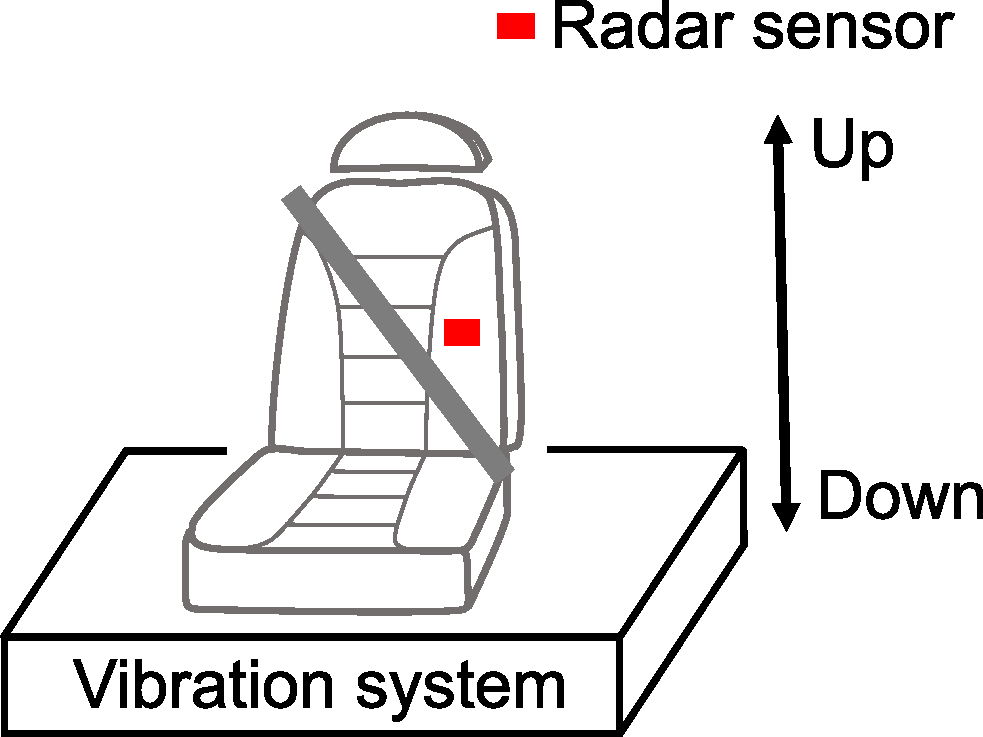
\includegraphics[width=0.7\columnwidth]{sensorstructure.pdf}
%  \vspace{0pt} % 図とキャプション間の余白調整
  \caption{Vibration measurement system and driver's seat with radar sensor.}
%  \vspace{-10pt} % キャプション下部の余白調整
  \label{fig:sensorstructure}
\end{figure}
%-%-%-%-%-%-%-%-%

%-%-%-%-%-%-%-%-%
\begin{figure}[tb]
  \centering
%  \vspace{0pt} % 図上部の余白調整
  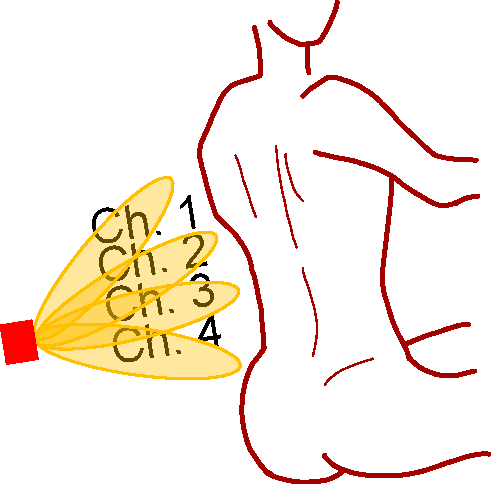
\includegraphics[width=0.4\columnwidth]{sensorimg.pdf}
%  \vspace{0pt} % 図とキャプション間の余白調整
  \caption{Beams from radar sensor for measurering back of driver's body.}
%  \vspace{-20pt} % キャプション下部の余白調整
  \label{fig:sensorimg}
\end{figure}
%-%-%-%-%-%-%-%-%


\section{振動測定系と測定条件}
\hspace{1.0em}

\subsection{振動測定系}
\hspace{1.0em}

本稿で仮定するレーダセンサの振動測定系はFig.~\ref{fig:sensorstructure}を示す.運転者を模した被験者が座った状態で振動測定系全体を上下方向に振動させる.Fig.~\ref{fig:sensorimg}に示す通り,レーダセンサを背部にあたるシートの内部に埋め込んでいるため,運転者の背部の体表面の微小変位を測定することが可能である.またFig.~\ref{fig:sensorimg}に示すように,4チャネルの異なる指向性レーダで駆動しているため,同時に近傍4点の体表面変位を測定した4~chの観測信号を得ることができる.

\subsection{レーダセンサの観測スペクトログラム}
\hspace{1.0em}

レーダセンサで観測された信号の内1~chのスペクトログラムをFig.~\ref{fig:1chobs}に示す.観測信号には心拍以外にも,振動台による振動成分及び呼吸に起因する体動成分等が混在していることが確認できる.そのため,本稿ではBSSを用いて心拍成分のみを抽出することを目指す.

また本稿では,分離した信号と比較する参照値を得るために,Zephyr Technology社の接触型心電図センサ(ECG)Bioharnessを用いてECG信号を取得している.心拍の参照値の計算には,このBioharness内部で実装されているアルゴリズムを用いる.Bioharnessの技術的な資料は公開されておらず原理は不明であるが,恐らく一般的な心拍推定アルゴリズムであるR-R間隔(R波と呼ばれる心拍波形の間隔)推定に基づくものと予想される.また,このECGセンサのサンプリング周波数は250~Hzである.接触型ECGセンサであるため,振動台の振動が加えられても高精度な心拍を得ることが可能である.本稿では,このECGセンサから得られる心拍と同程度の精度でレーダセンサの信号から心拍を推定することが目的となる.

%-%-%-%-%-%-%-%-%
\begin{figure}[tb]
  \centering
  \vspace{0pt} % 図上部の余白調整
  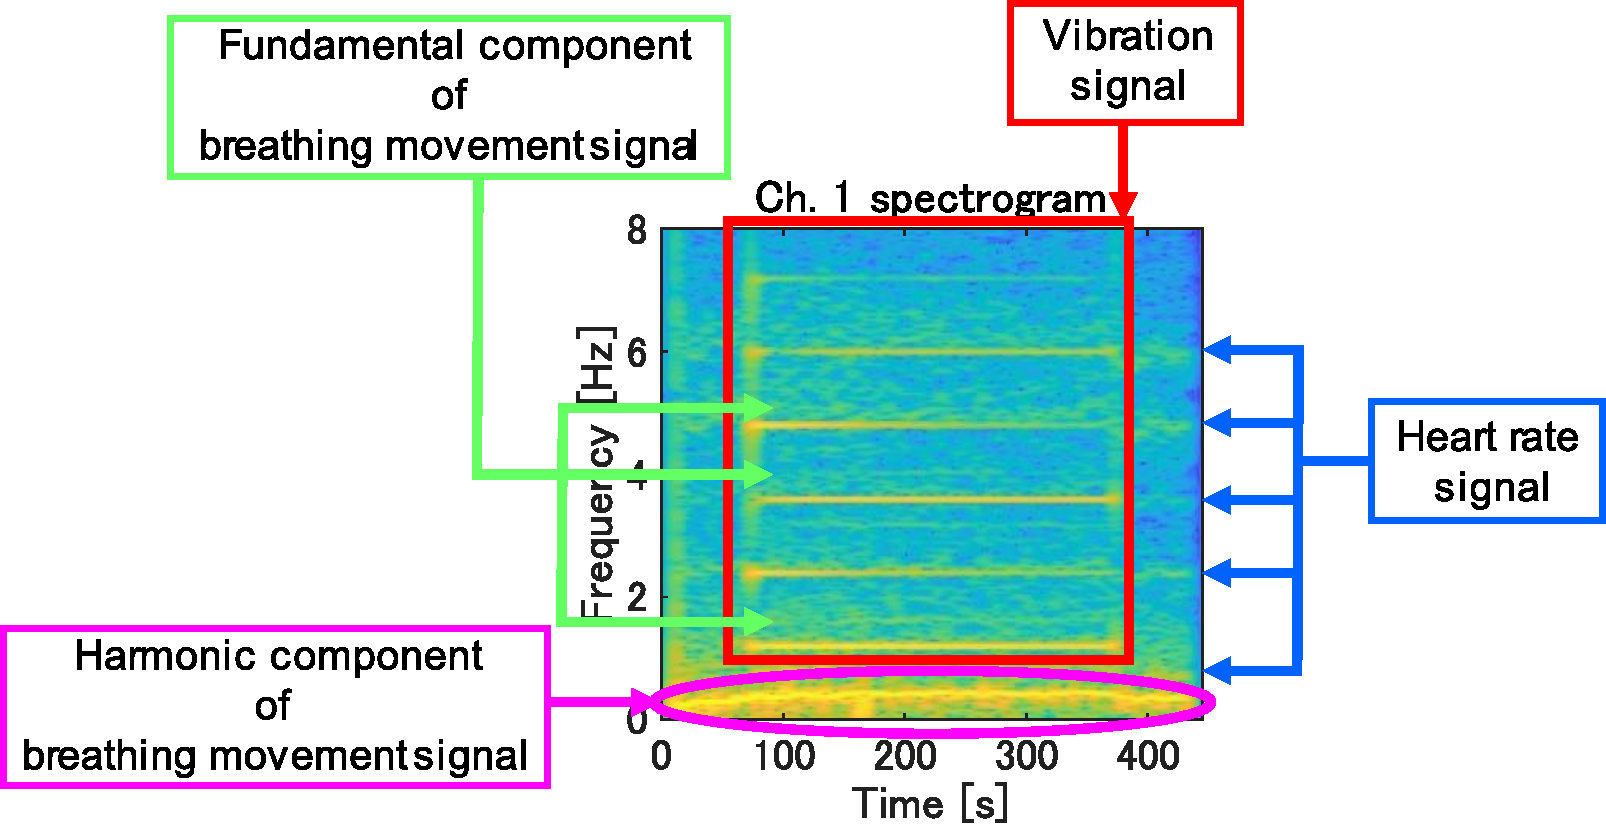
\includegraphics[width=1.0\columnwidth]{1chobsspect.pdf}
  \vspace{-20pt} % 図とキャプション間の余白調整
  \caption{Each component in first channel spectrogram obtained by radar sensor.}
  \vspace{-20pt} % キャプション下部の余白調整
  \label{fig:1chobs}
\end{figure}
%-%-%-%-%-%-%-%-%

\section{BSS及び心拍推定アルゴリズム}
\hspace{1.0em}

\subsection{IVA}
\hspace{1.0em}

\subsection{ISNMF}
\hspace{1.0em}

\subsection{ILRMA}
\hspace{1.0em}

\subsection{心拍推定アルゴリズム}
\hspace{1.0em}

\section{観測信号にフィルタを適用しない場合のBSS及び心拍実験}
\hspace{1.0em}

\subsection{実験条件}
\hspace{1.0em}

\subsection{実験結果}
\hspace{1.0em}

\section{観測信号にフィルタを適用した場合のBSS及び心拍推定実験}
\hspace{1.0em}

\subsection{前処理として適用するフィルタの設計}
\hspace{1.0em}

\subsection{実験条件}
\hspace{1.0em}

\section{実験結果}
\hspace{1.0em}

\section{結論}
\hspace{1.0em}

........

\section{出筆上の簡単な注意点}
\hspace{1.0em}
詳細は執筆要項をご覧下さい。

\subsection{原稿}
\hspace{1.0em}
原稿はワープロ等を用いて{\bf A4サイズ}で作成して下さい.
原稿は{\bf 6枚以内}です.
6枚を越えた原稿は受け付けませんので,ご注意下さい.
\underline{\bf 上下のマージンは25mm以上,左右のマージンは}\\
\underline{\bf 17mm以上}にして下さい.\\
上記の余白には何も記述しないでください.たとえば,ページ番号などです.

\subsection{文字の色・大きさ・フォント}
\hspace{1.0em}
文字は黒色を用いて下さい.(カラーは不可)
目安として表題16ポイント、著者名・所属・本文10.5ポイント以上をお使い下さ
い。

\subsection{図と表,写真}
\hspace{1.0em}
図と表:直接原稿中に張り込んでください.

\section{原稿提出方法}
\hspace{1.0em}
\underline{\bf Web上から電子的に提出してください。}\\
(URL: %%WSURL)\\
なお、印刷・製本スケジュールの関係上,提出期限後の原稿訂正,差し替えには応
じかねますので,ご注意下さい.

\section{問い合わせ先}
出版担当幹事までお願いします。

\vspace{13em}

\begin{thebibliography}{99}

\bibitem{abc} 著者名、``題目''
{\em 出典論文誌名}, Vol. XX, No. YY, pp.ZZ1-ZZ2, Dec., 1996

\bibitem{def} 著者名、``題目''
{\em 出典論文誌名}, Vol. XX, No. YY, pp.ZZ1-ZZ2, Dec., 1996

\end{thebibliography}

\end{document}
